\section{Experimental Results}

This chapter presents the experimental results of all proposed algorithms, regarding scalability, bucket cost balancing, the impact of different Sensitivity Analysis methods on reuse and the impact of the bucket size on run time.

\subsection{Experimental Environment}

We evaluated the proposed algorithms using a set of tissue images from brain cancer studies~\cite{kong2013machine}. The images were divided into 4K$\times$4K tiles for concurrent execution.  The image analysis workflow consisted of normalization, segmentation and comparison stages. The comparison stage computes the difference between masks generated and a reference mask set, created using the application default parameters. The experimental evaluations were conducted on two distributed memory machine environments. The first is the TACC Stampede cluster, with each node having dual socket Intel Xeon E5-2680 processors, an Intel Xeon Phi SE10P co-processor and 32GB RAM. The nodes are inter-connected via Mellanox FDR Infiniband switches. Stampede uses a Lustre file system accessible from all nodes. The second environment is the PSC Bridges cluster. Each node has a dual socket Intel E5-2695 and 128 GB RAM. Bridges uses a Pylon file system accessible from all nodes. The application and middleware codes were compiled using Intel Compiler 13.1 with ``-O3'' flag in both cases. All experiments were replicated at least 5 times and any claims for equivalence or difference between two algorithms of a given group were asserted through a t-test (two-tailed, not assuming homoscedasticity), on which $P < 0.001$ was chosen as the condition for assuming the difference to be statistically significant.

\subsection{Impact of Multi-level Computation Reuse for Multiple SA Methods} \label{sec:opt-search}

This section presents the impact of the computation reuse to the performance
of the MOAT and VBD SA methods. We first compute MOAT on all the application
parameters, because it demands a smaller per parameter sampling to exclude
those parameters that are non-influential to the output from the VBD. Most of
the experiments in this section were executed using a small number of machines,
because this section intended to detail the gains with the reuse optimizations.
However, Sections \ref{sec:bucket} and \ref{sec:scale} present experimental 
results for runs with large numbers of nodes.


\subsubsection{Impact of Multi-level Computation Reuse for MOAT}

Figure \ref{fig:reuse-overall} presents the execution times of MOAT studies
with parameter sample sizes varying from 160 to 640, which were executed using
only 6 Stampede nodes to demonstrate the impact of the optimizations. The parameters
were generated with a quasi-Monte Carlo sampling using a Halton sequence, which
is known to provide a good coverage of the parameter space. These experiments
use $MaxBucketSize$ set to 7, and the execution times refer to the makespan and
also include the cost to perform the computation reuse analysis and I/O.  
For the task level
merging approaches, the time spent by the merging algorithm is shown in the
upper part of the graph bars.  Additionally, five application versions were
executed: the ``No reuse'' that employs the replica based composition, the
``Stage level'' performs reuse only of stage instances, and the ``Task Level''
that reuses fine-grain tasks and is executed with the Na\"ive, SCA, and RTMA
algorithms. The TRTMA was not included on this analysis since for this scale it has the same performance as RTMA.

\begin{figure}[h]
\begin{center}
	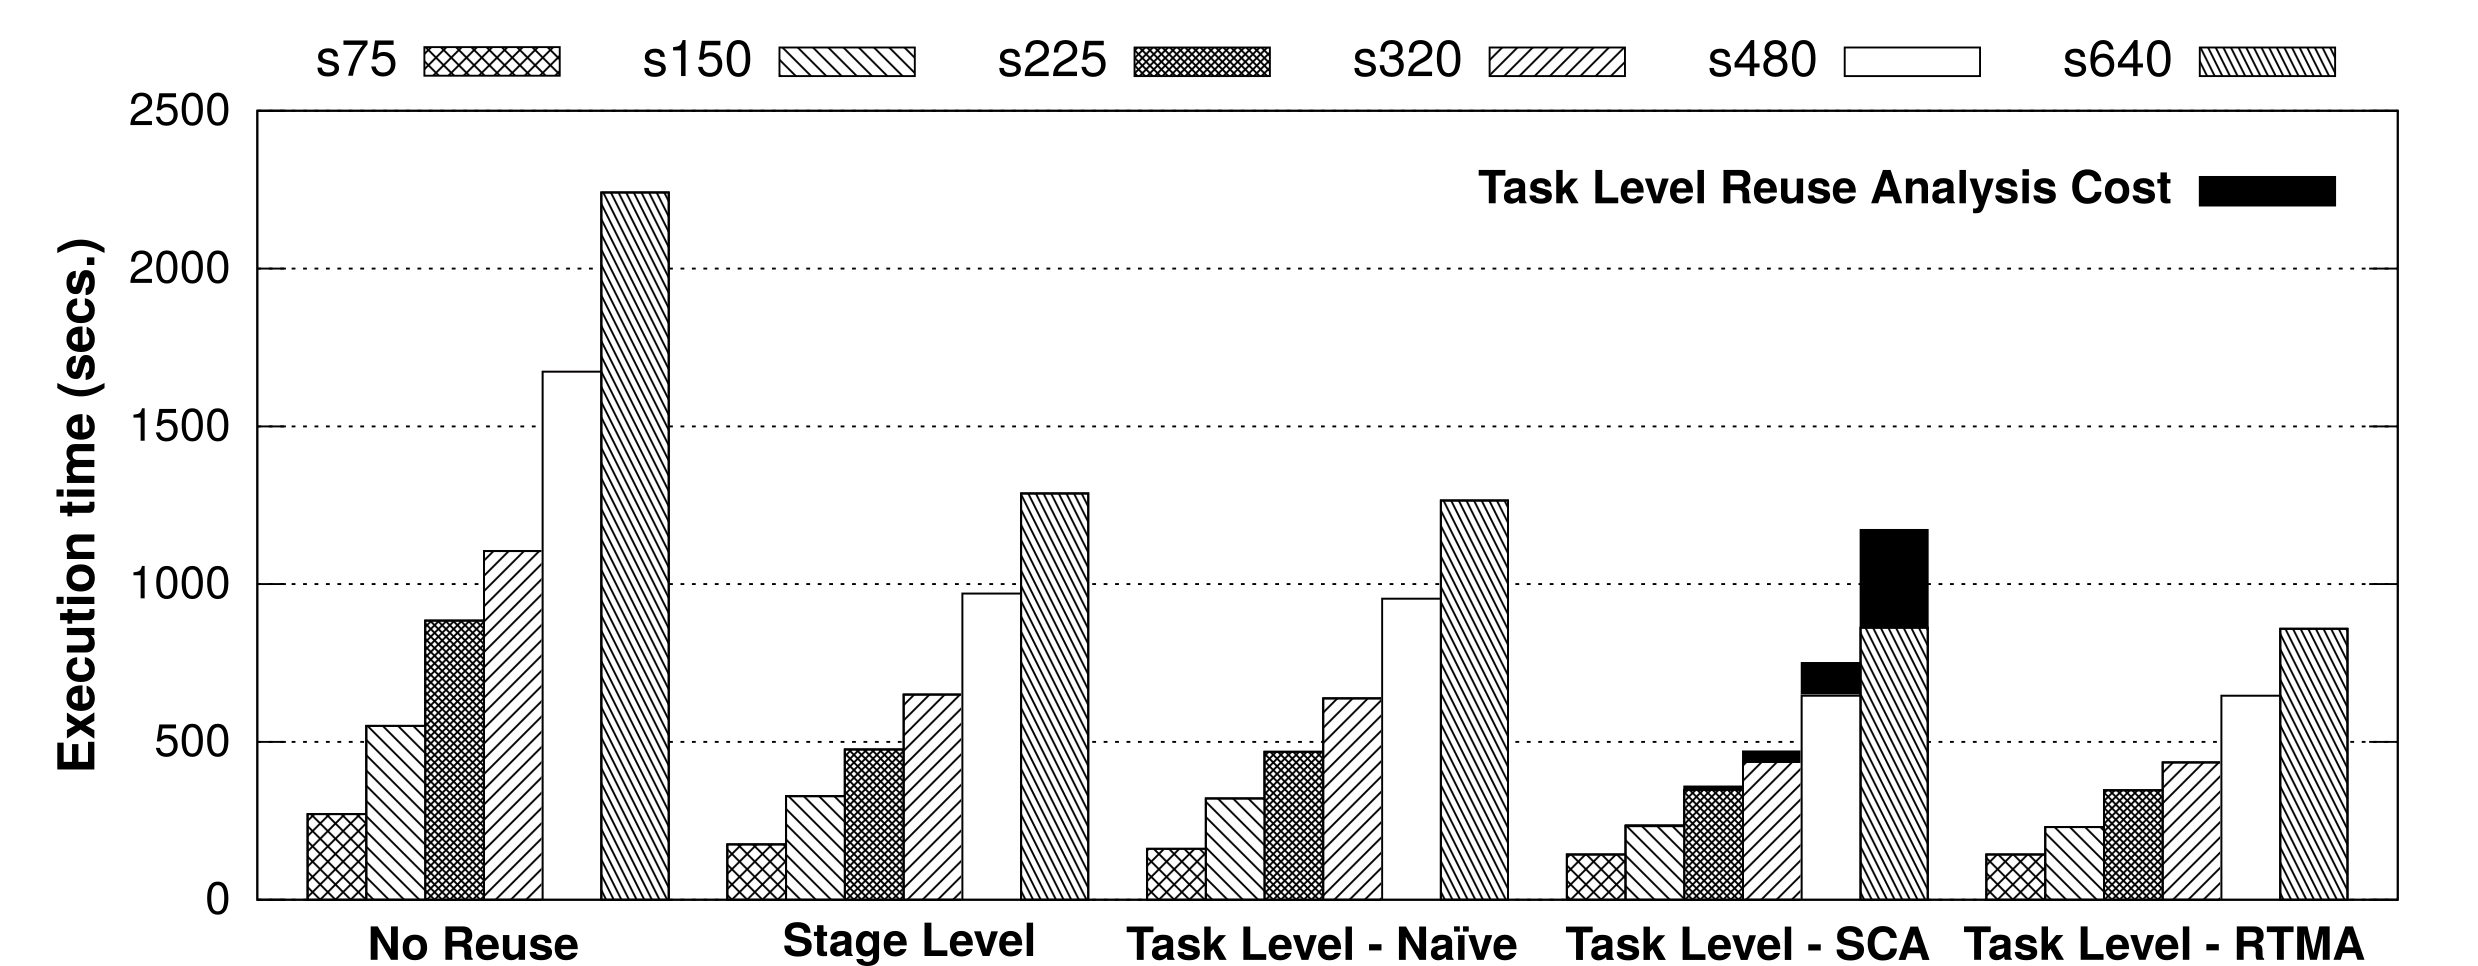
\includegraphics[width=1\textwidth]{img/moat-reuse}
	\caption{Impact of the computation reuse for different strategies as the sample size of the MOAT analysis is varied. E.g., s150 means that the experiment had 150 executions of the given workflow.}
	\label{fig:reuse-overall}
\end{center}
\end{figure}

The results presented in Figure~\ref{fig:reuse-overall} show that all application versions that reused computation significantly outperformed the baseline ``No reuse'' version. The ``Stage Level'' reached a speedup of up to 1.85$\times$ on top of the ``No reuse'', while the application versions with ``Task Level'' reuse have higher gains. The ``Task Level - Na\"ive'' is only slightly better than the ``Stage Level'' (1.08$\times$ faster in the best case, being statistically distinct based on a t-test). This result is attributed to the highly order dependent nature of the na\"ive approach. The ``Task Level'' with SCA and RTMA, on the other hand, have remarkable speedups of up to, respectively, 1.39$\times$ and 1.5$\times$ on top of the ``Stage Level'' reuse only. 

It is also noticeable from Figure~\ref{fig:reuse-overall} that the performance gains with RTMA increase as the sample size grows and, as a consequence, more reuse opportunities are available. In the SCA algorithm, however, the opposite behavior is observed. This is a result of the higher costs of executing SCA to compute the stages to be merged, which offsets the gains with the actual execution of the application after the merging. The time taken by Na\"ive, SCA, and RTMA to compute the reuse are shown on the top of their bars on Figure~\ref{fig:reuse-overall}. For a sample of size 640, the time taken by SCA is about 26\% of the entire execution. It is also interesting to see that although the RTMA takes a much shorter time to compute the merging choices, it provides solutions as good as the ones returned by the SCA. In the best case, RTMA attained a speedup of up to 2.61$\times$ on top of the ``No reuse'' version. 

Regarding the atained reuse on the tested algorithms, both SCA and RTMA achieved values around 33\% of reuse. This value is the raw value of tasks that were not executed due to a merging algorithm. As such, the speedup of 1.5$\times$ of RTMA on top of ``Stage Level'' reuse, which is greater than the 33\% of reuse, is justified by the variable cost of each task. This means that the of 33\% of tasks that were not executed, or reused, were comprised of expensive tasks. A further analysis on the costs of tasks and the impact this variance has on the implemented approaches is present on Section \ref{sec:task-cost}

\subsubsection{Impact of Multi-level Computation Reuse for VBD}

The performance of the proposed optimizations for the VBD are presented in
Figure \ref{fig:vbd}. The VBD was executed using the 8 remaining parameters
(the original parameter set contains 15 parameters) that were not discarded in
the MOAT analysis. VBD requirements are of the order of hundreds to thousands runs per
parameter. As such, the sample size in this experiment is higher and was varied
from 2000 to 10000 runs, whereas the same application versions used with MOAT
were evaluated. In order to accelerate this analysis, we have increased the
number of nodes to 16 Stampede nodes.

\begin{figure}[t]
\begin{center}
	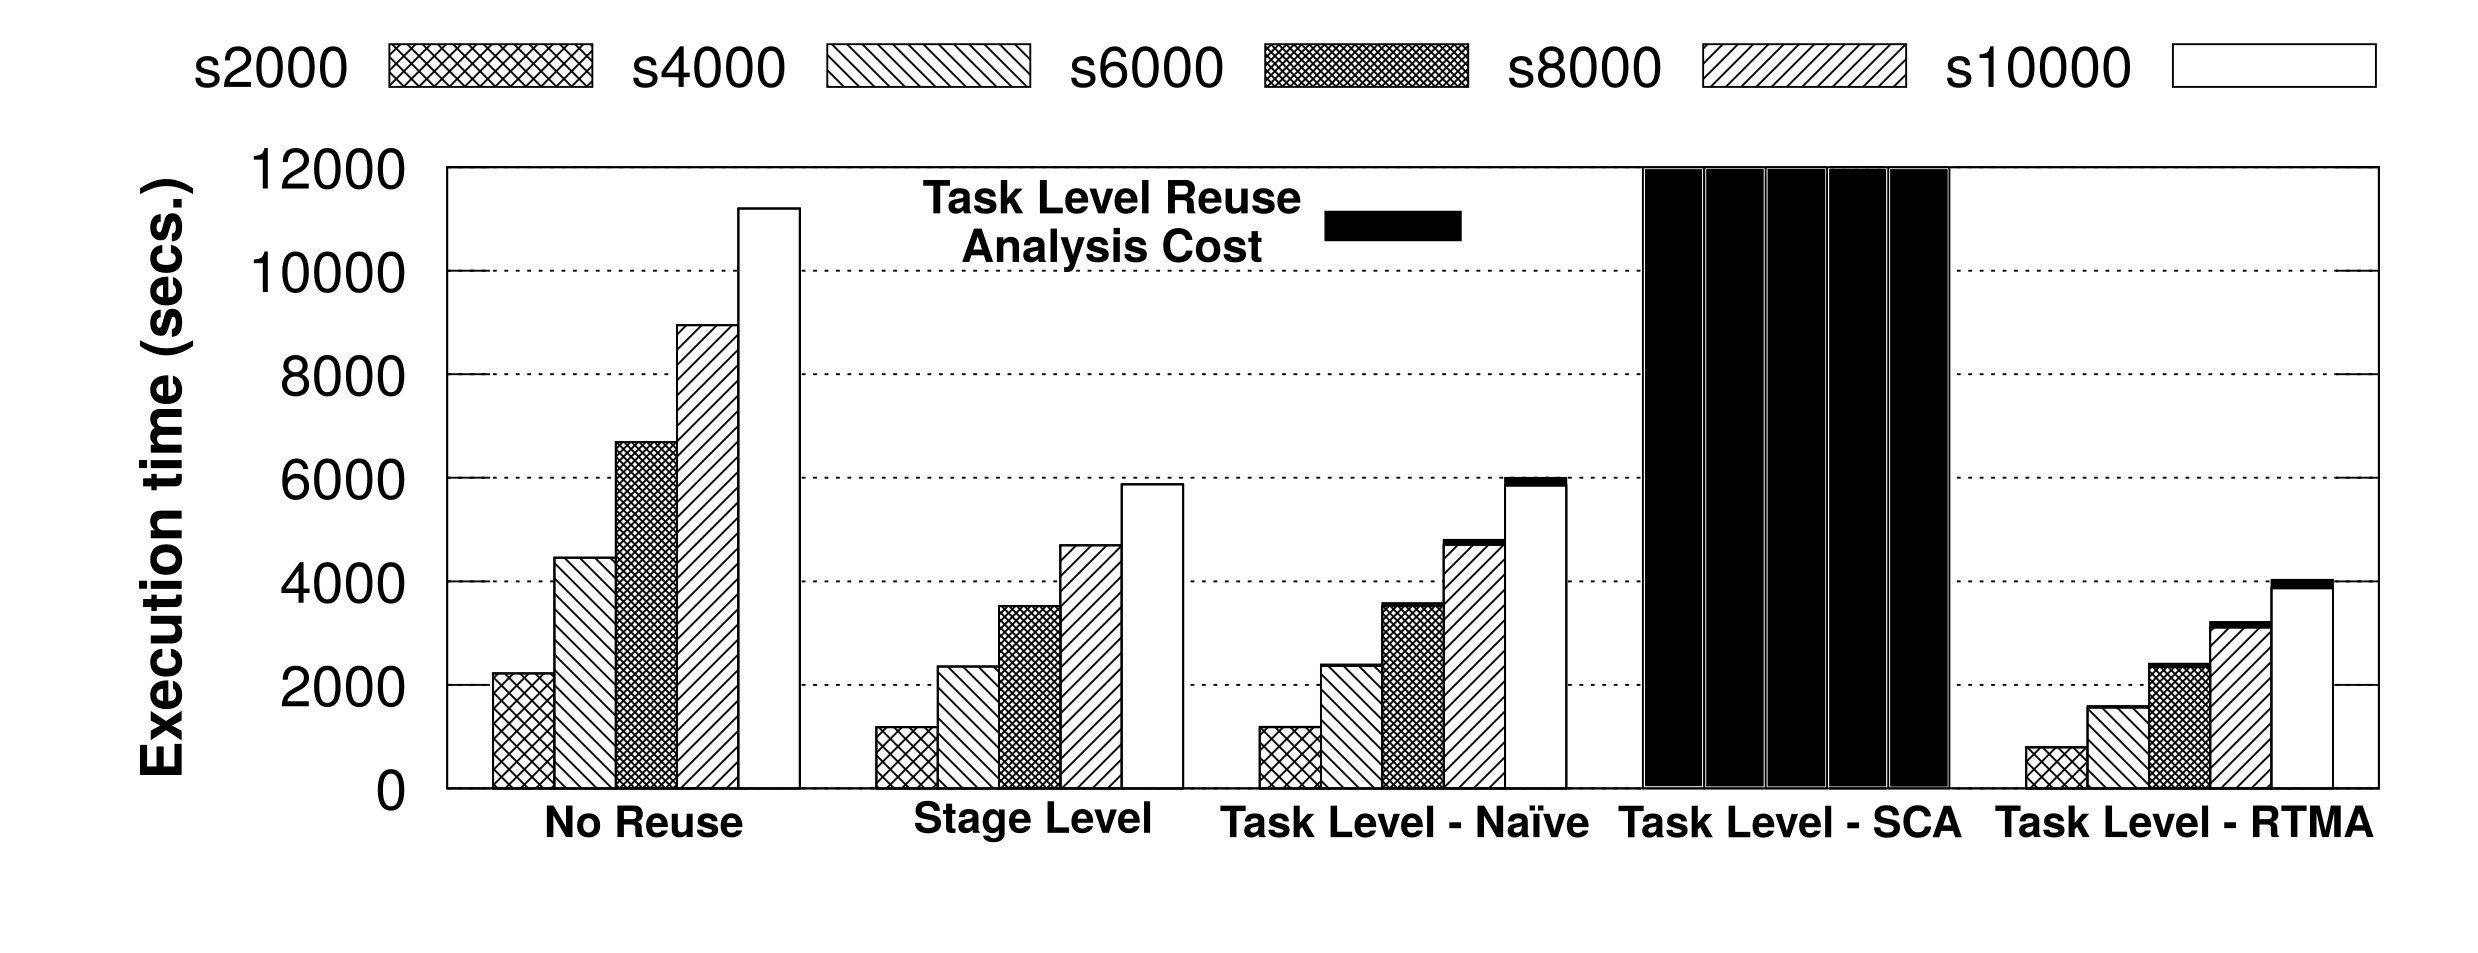
\includegraphics[width=1\textwidth]{img/vbd-reuse}
	\caption{Impact of the computation reuse strategies for the VBD SA method.}
	\label{fig:vbd}
\end{center}
\vspace*{-3ex}
\end{figure}

As presented in Figure \ref{fig:vbd}, the relative performance of the application versions is similar to that observed with MOAT, except for the task level merging using SCA. Given that the sample size used in VBD is much higher, the SCA was not even able to finish computing the reuse to start up the actual execution of the workflow in 14000 secs. The RTMA had speedups of at most 2.9$\times$ against the ``No Reuse'' approach, and 1.51$\times$ on top of ``Stage Level''. These speedups were consistent with the ones found in the MOAT analysis. Similarly, the reuse for the VBD experiments was of at most 35\% for 10000 executions for the RTMA.

\subsection{SA Methods Reuse Analysis}
\label{sec:methods_results}

For all previous computation reuse tests which used the VBD method, the experiments were generated with the Latin Hypercube Sampler (LHS). Since the computation reuse on this work is highly reliant on the generated experiments, some sensitivity analysis methods were analyzed regarding their maximum reuse potential. Among them, in addition to LHS, the Monte-Carlo (MC) and Quasi-Monte-Carlo (QMC) methods were analyzed. The results are presented in Table \ref{tab:sa_methods}. This analysis is only performed for VBD given its continuous ranges of parameter values, which would present itself with less potential reuse when compared to MOAT methods and their discrete parameter value ranges.

\begin{center}
\begin{table*}[h]%
\centering
\begin{tabular*}{250pt}{@{\extracolsep\fill}lccc@{\extracolsep\fill}}
\toprule
Sample Size	&	200	&	600	&	1000 \\
\midrule
MC	&	36.35\%	&	36.46\%	&	36.40\% \\
LHS	&	36.62\%	&	36.44\%	&	36.44\% \\
QMC	&	35.10\%	&	34.44\%	&	33.48\% \\
\bottomrule
\end{tabular*}
\caption{Maximum computation reuse potential for MC, LHS and QMC methods with different sample sizes. For VBD, the number of experiments is $10 \times SampleSize$. The reuse percentages represent fine-grain reuse after coarse-grain reuse, meaning that only fine-grain reuse is being shown.\label{tab:sa_methods}}
\end{table*}
\vspace*{-3ex}
\end{center}




\subsection{Impact of Max Bucket Size}
\label{sec:bucket}

This section presents the impact of varying the $MaxBucketSize$ parameter on the execution times. As shown in Figure \ref{fig:mbs}, an increase in $MaxBucketSize$ leads to smaller execution times because of the larger number of merging opportunities. This increase has, however, a threshold, after which the maximum reuse for the experiment is achieved (usually arround 33\% of reuse, which results in speedups close to 1.5$\times$).

However, it interesting to notice that the variation in execution times as a result of the bucket size changes, when comparing the two ends ($MaxBucketSize$ 2 and 8), is up to 12\%, which shows that ``Task Level'' reuse can achieve significant gains even with small bucket sizes. This is result shows the viability of fine-grain reuse for execution environments on which there is a limited amount of memory available.

A large-scale SA experiment using the sample size of 240, 4,276 4K$\times$4K image tiles, and 128 Stampede computing nodes, using all optimizations and the ``No reuse'', ``Stage Level'', and ``Task Level RTMA'' versions of the workflow attained execution times of, 15,681s, 12,544s and 6,173s, respectively.

\begin{figure}[h!]
\begin{center}
	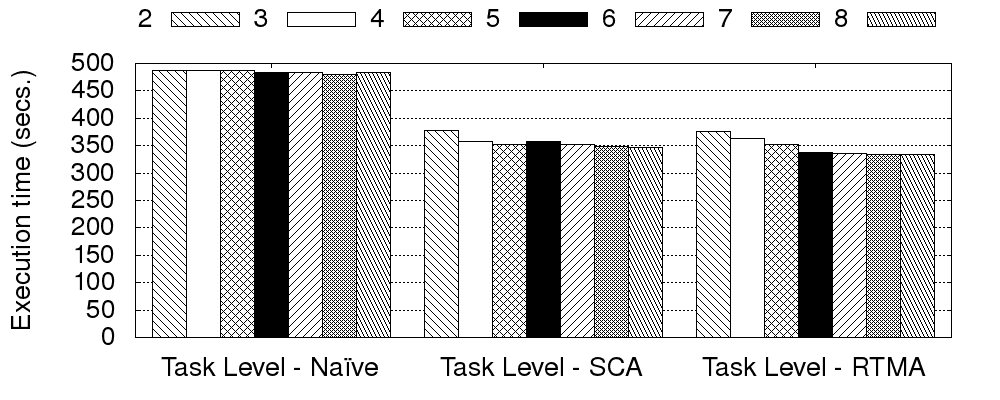
\includegraphics[width=0.9\textwidth]{img/mbs}
	\caption{Impact of varying $MaxBucketSize$ from 2 to 8.}
	\label{fig:mbs}
\end{center}
\vspace*{-3ex}
\end{figure}

It is important to highlight that the task level merging reduces the number of stage
instances up to $MaxBucketSize$ times, and the parallelism as a consequence. This
could affect the application scalability if the number of stage instances after
the merging was not sufficient to completely use the parallel environment.

% However, this is not the case in a large-scale SA, because the number of stages instances to be executed in a study is very high. For instance, a SA with a sample size of 240 and 4,276 4K$\times$4K image tile, as employed in the previous experiment, involves the execution of $240\times4276\times3$(stages) or about $3\times10^6$ stage instances. Its reduction by a factor of $MaxBucketSize$ during the merging will still lead to a configuration with sufficient stage instances to use the environment in the scale we are running (up to 128 nodes). We have experimentally validated it, and the scalability before and after merging has no significant difference when up to 256 nodes are used. We recognize, however, that if we continue to reduce the stage per node ratio, by either heavily increasing the number of nodes or reducing the number of executed stages, smaller values of $MaxBucketSize$ should be chosen, considering its impactinto the parallelism.

\subsection{The Effect of the Merging on Scalability}
\label{sec:scale}

This section evaluates the case on which performing merging operations may lead to poor scalability due to loss of parallelism. This problem is caused by the load imbalance of executing a different number of buckets on each node and can be triggered by either increasing the amount of merging performed or by increasing the number of nodes used. The later case was reproduced in Figure \ref{fig:scale-new} with the MOAT SA method and a sample size of 1000, with up to 256 Worker Processes/nodes (WP). 

\begin{figure}[h]
\begin{center}
    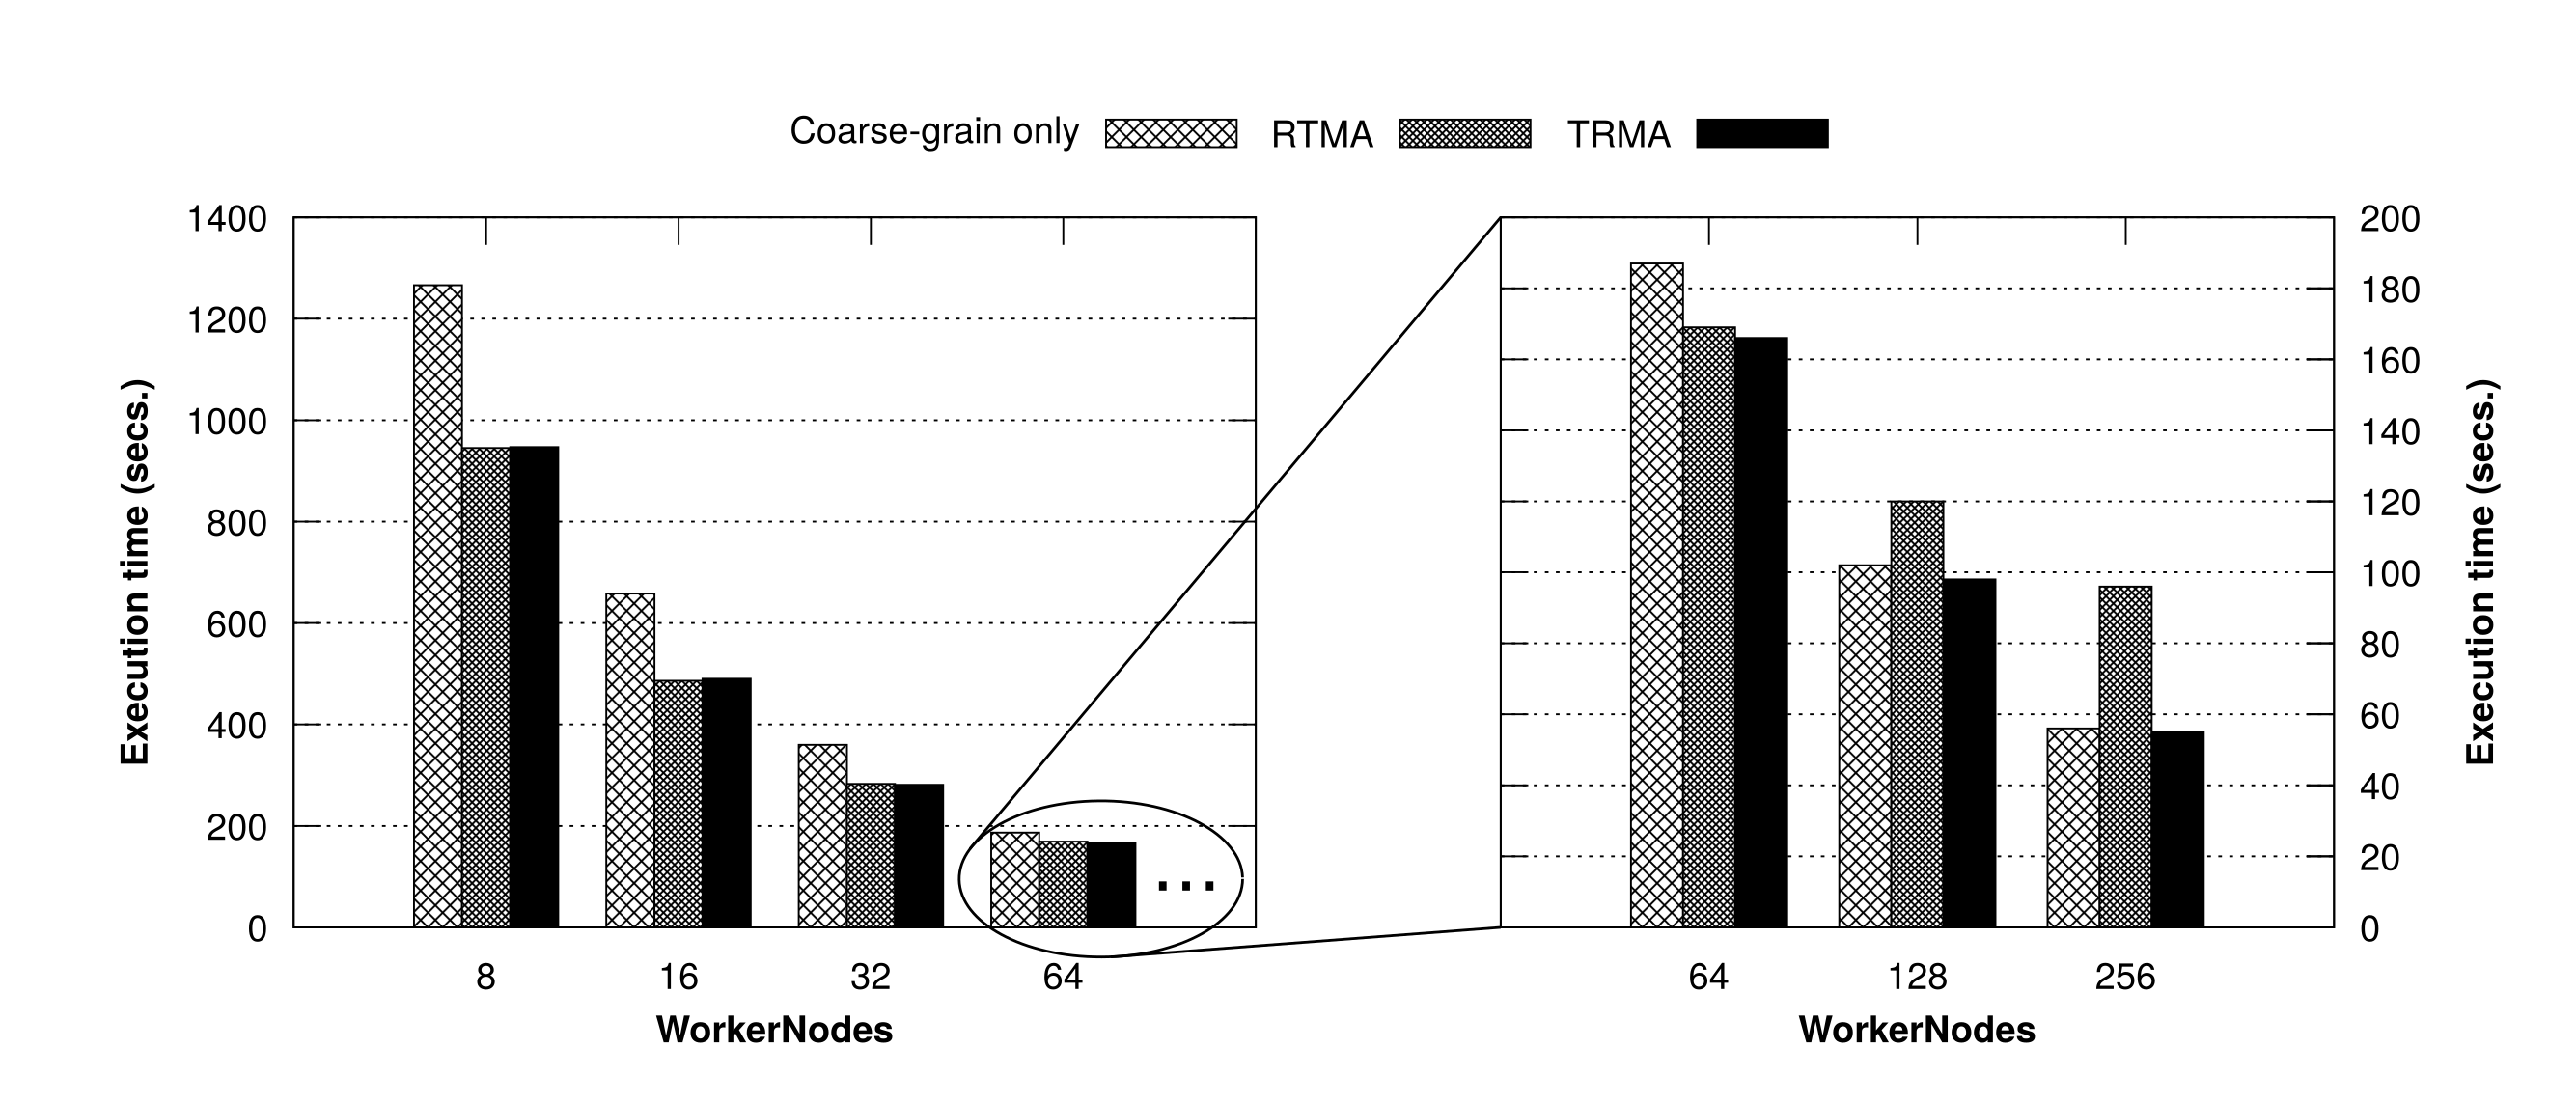
\includegraphics[width=1\textwidth]{img/scale-new}
	\caption{Comparison of the ``no fine-grain reuse'' (NR) approach with the RTMA and TRTMA. RTMA uses $MaxBucketSize$ 10, while TRTMA uses $MaxBuckets$ 3$\times$ the number Worker Processes (WP). The execution times for WP $>$ 32 were zoomed in a separated figure for the purpose of better visualization.}
	\label{fig:scale-new}
\end{center}
\vspace*{-3ex}
\end{figure}

This performance degradation caused by excessive merging, as seen with the parallel efficiency of the RTMA on Figure \ref{fig:srs2}, is aggravated by the variable cost of different buckets generated by the RTMA. The workflow used on this work had its stages broken into finer-grain tasks in order to mitigate this variance on the costs. Since the RTMA generate buckets that are balanced stage-wise, but not task-wise, this difference in the number of tasks per bucket may lead to imbalance on environments with a low stages-per-worker ratio. This imbalance leads to a reduction of parallelism and, thereafter, degradation on the performance of the application due to load imbalance among nodes. On these cases the Task-Balanced Reuse-Tree Merging Algorithm (TRTMA) could be employed to extenuate this problem.

\begin{figure}[h]
\begin{center}
    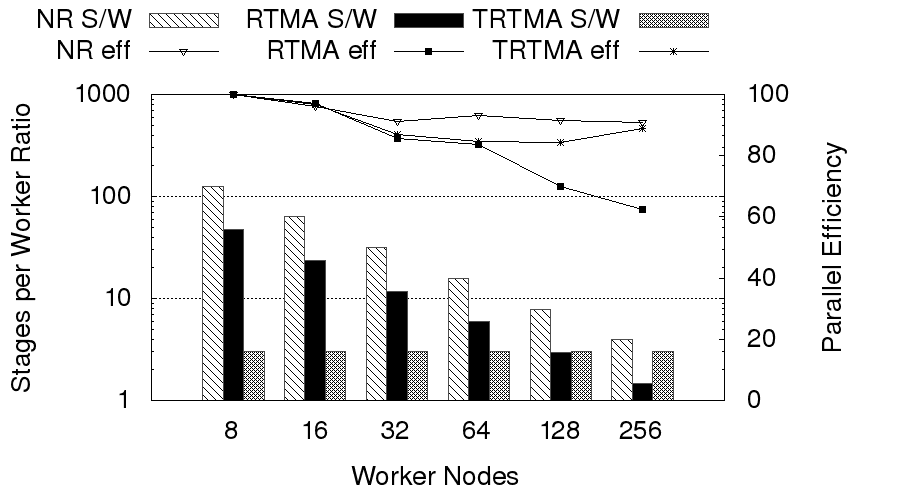
\includegraphics[width=1\textwidth]{gnuplot/eff.png}
	\caption{Combination of Stages per Worker Processes (S/W) and parallelism efficiency values. The S/W ratio for TRTMA was fixed as 3 for all WP values. The parallelism efficiency was calculated based on the previous execution (e.g. for WP 64, it is the execution time for WP 32 vs WP 64).}
	\label{fig:srs2}
\end{center}
\vspace*{-3ex}
\end{figure}

% \begin{center}
% \begin{table*}[t!]%
% \centering
% \begin{tabular*}{460pt}{@{\extracolsep\fill}lcccccccc@{\extracolsep\fill}}
% \toprule
% Worker Processes (WP)&	8		&	16		&	32		&	64		&	128		&	256		\\
% \midrule
% No Reuse S/W		&	126		&	63		&	31.5	&	15.75	&	7.85	&	3.93	\\
% RTMA S/W			&	47.25	&	23.62	&	11.81	&	5.9		&	2.95	&	1.47	\\
% \midrule
% No Reuse efficiency	&	-		&	96.21\%	&	91.26\%	&	93.03\%	&	91.43\%	&	90.95\% \\
% RTMA efficiency		&	-		&	97.20\%	&	85.72\%	&	83.64\%	&	70.08\%	&	62.44\% \\
% TRTMA efficiency		&	-		&	96.68\%	&	86.94\%	&	84.65\%	&	84.38\%	&	89.04\% \\
% \bottomrule
% \end{tabular*}
% \caption{Combination of Stages per Worker Processes (S/W) and parallelism efficiency values. The S/W ratio for TRTMA was fixed as 3 for all WP values. The parallelism efficiency was calculated based on the previous execution (e.g. for WP 64, it is the execution time for WP 32 vs WP 64). \label{tab:srs}}
% \end{table*}
% \vspace*{-3ex}
% \end{center}

\begin{center}
\begin{table*}[b]%
\centering
\begin{tabular*}{460pt}{@{\extracolsep\fill}lcccccccc@{\extracolsep\fill}}
\toprule
Worker Processes (WP)&	8		&	16		&	32		&	64		&	128		&	256	\\
\midrule
Speedup TRTMA vs NR	&	1.33	&	1.34	&	1.27	&	1.12	&	1.04	&	1.01	\\
\midrule
TRTMA reuse			&	32.96\%	&	32.96\%	&	32.11\%	&	30.58\%	&	28.23\%	&	10.73\%	\\
\bottomrule
\end{tabular*}
\caption{Speedup of the TRTMA vs the ``No Reuse'' (NR) approach. \label{tab:speedup}}
\end{table*}
\vspace*{-3ex}
\end{center}

Still on Figure \ref{fig:srs2} it is visible that if the stages-per-worker ratio becomes low enough, the RTMA parallel efficiency drops to an extent on which it performs worse than not performing any fine-grain reuse at all. The values of stages-per-worker ratio (S/W), parallel efficiency and TRTMA reuse, compiled on Figure \ref{fig:srs2}, show that regardless the reuse algorithm employed, for the highest WP values the S/W ratio becomes low enough to impact the parallelism. This is true not only to RTMA, which becomes worse than ``No Reuse'' (NR) after WP 64, but also for NR itself. This loss of parallelism in NR is an indication of the imbalance between stages without reuse caused by the variance on the cost of tasks of the same level, but different inputs. Given that, the NR parallel efficiency values can be seen as the upper bound for any approach, since the reuse degree cannot increase for bigger WP values, nor can the parallel efficiency.

The TRTMA approach manages to improve on the RTMA parallel efficiency through bucket balancing, resulting in it not becoming worse than NR (see Figure \ref{fig:srs2} and Figure \ref{fig:scale-new}). The speedups that TRTMA achieves on top of NR lowers as WP increases, becoming negligible for WP values of at least 128 (see Table \ref{tab:speedup}). Given that for WP 256 the TRTMA attained 10.73\% of reuse, the speedup should either match this value or come close to it. This phenomenon of lack of performance is cause by another source of imbalance on buckets.


\subsubsection{The Impact of Variable Task Cost}
\label{sec:task-cost}

By taking another look at Figure \ref{fig:srs2} we can notice that the loss of parallelism due to imbalance starts at WP 32 for the RTMA and TRTMA approaches. This indicates that there exists another source of imbalance, for merging algorithms only, that affects RTMA harder than TRTMA and that is unaffected by TRTMA balancing techniques. It was found that this imbalance comes from the difference in the cost of tasks of different levels.

\begin{center}
\begin{table*}[b]%
\centering
\begin{tabular*}{460pt}{@{\extracolsep\fill}lcccccccc@{\extracolsep\fill}}
\toprule
Task 				&	t1	&	t2	&	t3	&	t4	&	t5	&	t6	&	t7	&	Total\\
\midrule
Avg Exec Time (s)	&	1.14	&	1.99	&	0.65	&	0.33	&	0.76	&	3.76	&	0.86	&	9.51	\\
Percentual			&	12.03\%	&	20.90\%	&	6.92\%	&	3.49\%	&	8.02\%	&	39.59\%	&	9.05\%	&	100\%	\\
\bottomrule
\end{tabular*}
\caption{An empirical evaluation on the costs of each task of which a stage is composed of. This approximation was generated with the purpose of showing the relative cost of the tasks, not being suitable as a absolute cost approximation. \label{tab:profile}}
\end{table*}
\vspace*{-3ex}
\end{center}

As shown in Table \ref{tab:profile}, the costs of the task which compose a stage are not constant. As such, buckets which are balanced by the number of tasks may still be susceptible to imbalance. An example of such case is presented in Figure \ref{fig:unbal-ex}. There, we have two buckets with the same number of tasks, but with different topologies. The first bucket was generated with three stages that attained maximum reuse, while the second had only two stages with less reuse. By using the TRTMA, the difference of execution cost between them of around 25\% would go unnoticed. This imbalance is enough to impact the parallel efficiency of an application through load imbalance. Effectively, this problem just makes the imbalance of buckets by tasks visible on an earlier S/W ratio.

\begin{figure}[t!]
   \centering
   \begin{subfigure}[t]{0.9\textwidth}
       \centering
       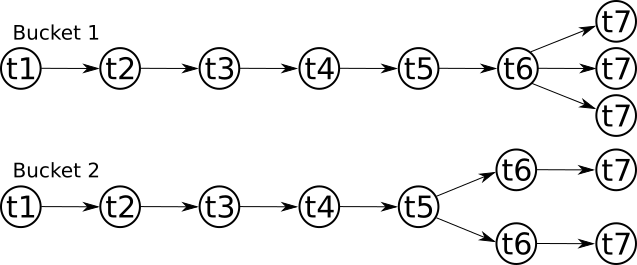
\includegraphics[width=0.7\textwidth]{img/unbal}
       \caption{Two example buckets and their reuse trees. Bucket 1 was the result of the merger of three stages, while Bucket 2 had two stages initially.}
       \label{fig:unbal}
   \end{subfigure}
   \par\bigskip
   \begin{subfigure}[t]{0.9\textwidth}
   	   \centering
	   \begin{tabular*}{400pt}{@{\extracolsep\fill}lcccccccc@{\extracolsep\fill}}
			\toprule
			Task 				&	t1	&	t2	&	t3	&	t4	&	t5	&	t6	&	t7	&	Total\\
			\midrule
			Bucket 1	&	0.12	&	0.20	&	0.06	&	0.03	&	0.08	&	0.39	&	0.27	&	1.18	\\
			Bucket 2	&	0.12	&	0.20	&	0.06	&	0.03	&	0.08	&	0.79	&	0.18	&	1.48	\\
			\bottomrule
	   \end{tabular*}
		\caption{Sum of relative costs of tasks for each bucket. For a bucket containing only a single stage, and thus 7 tasks, the total cost would be 1.}
		\label{fig:unbal-tab}
	\end{subfigure}
	   \caption{An example case on which two buckets with the same number of tasks have different execution costs. This is due to the difference in the cost of different tasks. In this example Bucket 1 should execute 1.25$\times$ faster than Bucket 2.}
   \label{fig:unbal-ex}
\end{figure}

Altogether, three sources of imbalance affects the maximum achievable parallel efficiency: (i) differently sized buckets (same stage count but different task count), (ii) buckets with the same size (task count) but different topologies, and (iii) same tasks having variant execution costs, which happens if two stages with the same topology and task count can have significantly different costs. The (i) problem is already solved by the TRTMA, while (ii) and (iii) can only be solved if we have an approximation of the costs of each task {\it a priori}.

%----------------------------


% \begin{figure}[t!]
% \begin{center}
%     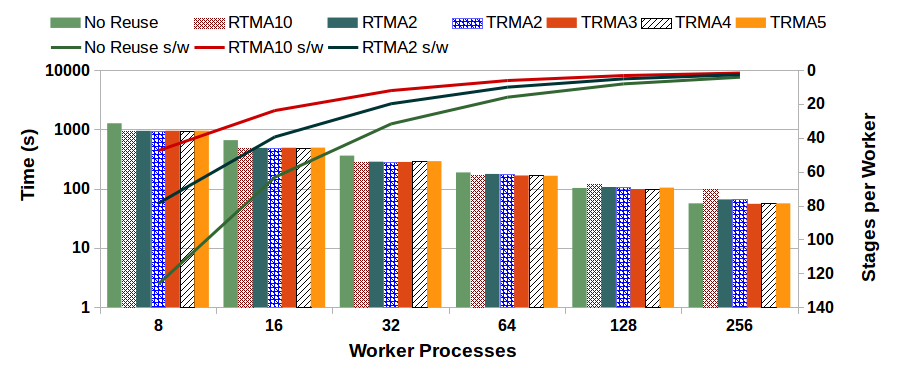
\includegraphics[width=0.9\textwidth]{img/scale-s1000-time-full}
% 	\caption{Comparison of the Coarse-grain-only approach with the RTMA and TRTMA. RTMA uses $MaxBucketSize$ 10 and 2, while TRTMA uses $MaxBuckets$ 2, 3, 4 and 5 $\times$ the number Worker Processes. The stages-per-worker ratio is also shown for the No Reuse and RTMA approaches only, since the ratios for TRTMA are fixed (2, 3, 4 and 5, respectively).}
% 	\label{fig:scale1000}
% \end{center}
% \vspace*{-3ex}
% \end{figure}

% Figure \ref{fig:scale1000} shows that when the ratio of stages per worker is low enough (manipulated here by increasing the number of workers) the RTMA stops to scale. This problem is so severe that when comparing the RTMA (with $MaxBucketSize$ 10) and ``No Reuse'' approaches, RTMA needs 74\% more time to execute 36\% less tasks on 256 Worker Processes. The RTMA (with $MaxBucketSize$ 10) performance drops from 128 Worker Processes on, when the stages-per-worker ratio is at least 3. By setting the stages-per-worker ratio to 3 we can see that the TRTMA outperforms all other approaches and configurations. This result is only achievable for two reasons, (i) the reuse achieved by using the TRTMA with $MaxBuckets$ $3 \times WorkerProcesses$ is high enough to reduce the overall execution cost (see Table \ref{tab:reuse}), (ii) while maintaining the buckets balanced task-wise.


% \begin{center}
% \begin{table*}[h]%
% \centering
% \begin{tabular*}{460pt}{@{\extracolsep\fill}lcccccccc@{\extracolsep\fill}}
% \toprule
% MaxBuckets	&	768	&	512	&	256	&	128	&	64	&	32	&	16	&	8	\\
% \midrule
% Reuse	&	10.73\%	&	26.06\%	&	30.61\%	&	31.01\%	&	32.95\%	&	32.98\%	&	33.89\%	&	33.91\%	\\
% \bottomrule
% \end{tabular*}
% \caption{Reuse of the TRTMA with different $MaxBuckets$ values.\label{tab:reuse}}
% \end{table*}
% \vspace*{-3ex}
% \end{center}

% Figure \ref{fig:scale1000} also shows how carefull we must be when chosing a stages-per-worker ratio value for TRTMA. By going too high the amount of reuse will be reduced. However, if the value is too low the amount of achievable reuse increases while unbalancement becomes a problem still. This unbalancement, while not being as bad as the one present in RTMA, is a consequence of the variable cost of tasks and cannot be easily solved, since it would require the computational cost of the tasks \textit{a priori}.

%----------------------------

% Given that the RTMA could not directly resolve balancement issues it was expected that there may exist some cases on which its use would result in such unbalancement that even the use of coarse-grain-only reuse would be better. On these cases the Task-Balanced Reuse-Tree Merging Algorithm (TRTMA) could be employed to extenuate this problem. One of this cases was found by using the MOAT SA method with a sample size of 1000 and up to 256 Worker processes/nodes. 

% Another way to present this information is to plot the product of the makespan of the application by the number of worker processes needed (see Figure \ref{fig:scale1000-2}). This can be seen as a crude analogy to the overall system time (i.e., the time needed by all processor cores). As we scale up the available resources this average time increases due to the overhead of executing the application parallel. On a perfectly scalable system all averages would have the same value. The ``No Reuse'' approach has an increase on the average time of at most 1\% as we scale up the number of workers from 8 to 64, and at most 10\% from 64 to 256 workers. This shows that there is some unbalancement between stages with the same number of tasks, which can only be addressed if the actual cost of each task given their input parameters was considered.

% \begin{figure}[t!]
% \begin{center}
%     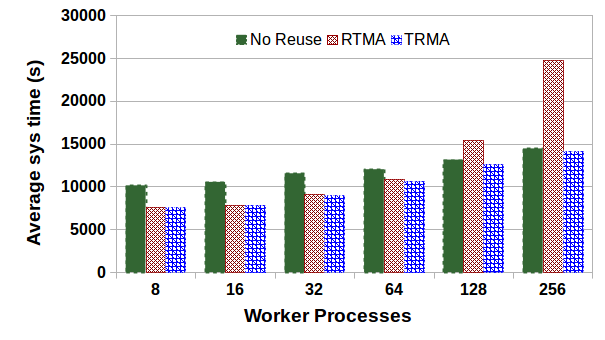
\includegraphics[width=0.8\textwidth]{img/scale-s1000-avg-t}
% 	\caption{Comparison of the Coarse-grain-only approach with the RTMA and TRTMA.}
% 	\label{fig:scale1000-2}
% \end{center}
% \vspace*{-3ex}
% \end{figure}

% Still on Figure \ref{fig:scale1000-2}, the unbalancement cost becomes rather visible on the RTMA, which has the same under-1\% scalability overhead for 8 to 16 workers, going up to 60\% when scaling from 128 to 256 workers. The TRTMA stays between the RTMA and ``No Reuse'' scalability-wise. Also, the TRTMA has an increase in the average time of 12-18\% across all worker scaling values, which is not necessarily an issue given that for 8 workers TRTMA executes the application in 74\% of the ``No Reuse'' time, while reaching a marginal speedup of 1.01 for 256 workers, again, comparing with ``No Reuse''. Lastly, these results show that the TRTMA can behave like the RTMA when the stages-per-core ratio is high, while not degrading its performance on lower stages-per-core ratio situations.

% The results of Figure \ref{fig:scale800} can be split in three moments. The first one, when the number of cores is at most 56, the number of stages per core is still high enough for RTMA to avoid unbalancement issues. At this time, both RTMA and TRTMA have similar performances. As we move further, when the number of cores is between 56 and 112, RTMA's scalability starts to drop as TRTMA and Coarse-grain only keep scaling. It is worth noting that on this interval the experimental values of TRTMA and Coarse-grain only are equivalent with a degree of confidence of 90\%. The final range, with the number of cores of at least 140 shows RTMA runtime reaching a limit, given its unbalancement. As for TRTMA and Coarse-grain, their equivalence now reaches a degree of confidence of 95\%, thus showing that the TRTMA can achieve the same reuse optimization of RTMA when the issue of unbalancement is inexistent (i.e., large scale of experiments / executions) while not degrading it's performance on these extreme low-scale settings (low number of stages per cores).
























% Up to this moment this work has already presented results on which fine-grain computation reuse lead to speedups to up to 1.5$\times$ on top of the coarse-grain reuse algorithm. In the rest of this work we plan to optimize the reuse of computation as follow:

% \paragraph{1. Investigate clustering algorithms:}
% In order to further the understanding of fine-grain computation reuse and also maximize the speedup achievable through fine-grain reuse, new ways to model the fine-grain reuse problem shaw be researched. One promising way is to attempt to model the problem as a clustering problem, which has a plenitude of mature material. The fine-grain reuse problem can be modeled as a bag of stages with different degrees of reuse among themselves, which must be divided into clusters of stages. By using some variation of the reuse degree equation as a way to calculate the distance between stages we can employ a Fuzzy C-Means clustering algorithm to search for stage merging solutions.

% \paragraph{2. Optimize the RTMA:} Another way to improve the fine-grain reuse performance is by optimizing the best algorithm found so far, the RTMA. A possible optimization involves performing two-level-aware pruning in order to take advantage of more intrinsic reuse opportunities. These missed opportunities exist due to possible misalignment of stages after the move-up operation. Figure \ref{fig:bad-ex} demonstrates this case, on which ideally, nodes $c$ and $d$ should remain together but are instead placed into different buckets due to bad ordering of stages. Another reason for this misalignment is the loss of reuse information after the move-up operation, on which the reuse information of stage instances pairs $a$ and $b$, and $c$ and $d$ do not exist on Figure \ref{fig:bad2}, after the move-up operation happens.

% \begin{figure}[h]
%    \centering
%    \begin{subfigure}[b]{0.45\textwidth}
%        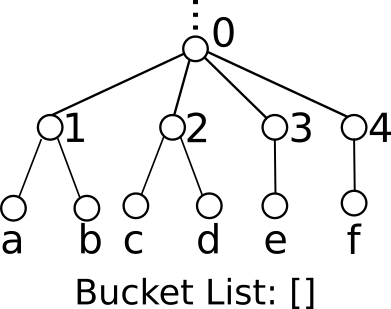
\includegraphics[width=\textwidth]{img/bad1.png}
%        \caption{Initial reuse subtree.}
%        \label{fig:bad1}
%    \end{subfigure}
%    \hspace{3mm}
%    \begin{subfigure}[b]{0.45\textwidth}
%         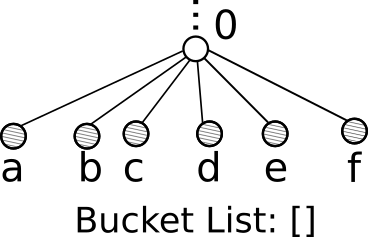
\includegraphics[width=\textwidth]{img/bad2.png}
%         \caption{Reuse subtree after move-up operation, enabling stages $a$-$f$ to be divided into two buckets.}
%         \label{fig:bad2}
%     \end{subfigure}
%     \par\bigskip
%     \begin{subfigure}[b]{0.6\textwidth}
%         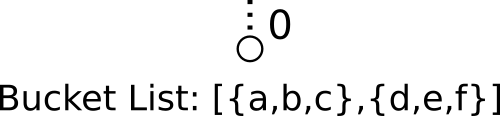
\includegraphics[width=\textwidth]{img/bad3.png}
%         \caption{Sub-optimal merging result, separating $c$ form $d$.}
%         \label{fig:bad3}
%     \end{subfigure}
%     \caption{An example of Reuse Tree based merging with MaxBucketSize 3 with sub-optimal results.}
%     \label{fig:bad-ex}
% \end{figure}

% \paragraph{3. MaxBucketSize system based definition:} As seen on preliminary testing, the $MaxBucketSize$ value is influential on the attained speedup of fine-grain merged executions. Given that this value is a limit used to ensure that merged stages can be executed on the given environment, regarding the system memory, $MaxBucketSize$ will be calculated automatically, using the characteristics of both the underlying infrastructure and the workflow to be executed.

% \paragraph{4. Large scale testing:} Finally, further testing should be done on lager scale, both with more hardware resources and larger experiments. It is also interesting that other SA methods are used (e.g., VBD).

% \paragraph{5. Write a periodic article:} Finishing the aforementioned activities, write and submit a periodic article containing the RTMA fully optimized and the new clustering algorithm, tested on large scale.